\section{Stage}

\subsection{But}
Le but de ce travail est de proposer un algorithme efficace de compression et d'indexation des reads peu gourmand en mémoire. Pour cela, la piste privilégiée est l'étude de la transformée de Burrows-Wheeler à contexte borné. 

Les reads étant une donnée très redondante, la recherche d'un motif dans le texte devrait occasionner de nombreux calculs identiques. L'un des objectifs est donc d'optimiser la recherche en factorisant ces calculs. 

De plus, du fait de la redondance des données, les $k$-contextes devraient être grands et nombreux. Nous allons donc essayer d'accroître la probabilité d'obtenir de longues suites de caractères identiques.


\subsection{Approche}
%Pour augmenter les suites de caractères identiques, l'idée est de trier la \kbwt\ sur ses $k$-contextes. Il faut donc aussi fournir les structures et algorithmes nécessaires au maintien des propriétés de la \bwt\ sur la \kbwt\ triée.
%La redondance des calculs dans la recherche des positions de motif est elle évitée grâce à un nouvel algorithme qui parcourt la fonction LF() \textit{par blocs}.
%Enfin, une autre amélioration sur la taille de l'espace utilisé pour la \kbwt\ est effectuée grâce au stockage de la fonction LF().

\subsubsection{Tri dans les k-contextes}
Nous proposons de trier la \kbwt\ sur ses $k$-contextes, comme dans la figure \ref{tri}, pour accroître le nombre et la taille des suites de caractères identiques.

\begin{figure}[h!]
\fbox{%
  \begin{minipage}{\linewidth}
    t = "\textsc{ananaaanaanaa\$}"
  	\begin{center}
  	  \textsc{%
    \$an anaaanaana {\color{lightgray}a} a\\
    a\$a nanaaanaan {\color{lightgray}a} a\\
	aa\$ ananaaanaa {\color{lightgray}n} n\\
	aaa naanaa\$ana {\color{lightgray}n} n\\
	{\color{red}aan} aanaa\$anan {\color{lightgray}a} a\\
	{\color{red}aan} aa\$ananaaa {\color{lightgray}n} a\\
	{\color{blue}ana} naaanaanaa {\color{lightgray}\$} \$\\
	{\color{blue}ana} aanaanaa\$a {\color{lightgray}n} a\\
	{\color{blue}ana} anaa\$anana {\color{lightgray}a} a\\
	{\color{blue}ana} a\$ananaaan {\color{lightgray}a} n\\
	{\color{green}naa} anaanaa\$an {\color{lightgray}a} a\\
	{\color{green}naa} naa\$ananaa {\color{lightgray}a} a\\
	{\color{green}naa} \$ananaaana {\color{lightgray}a} a\\
	nan aaanaanaa\$ {\color{lightgray}a} a
	  }
	\end{center}
	$k = 3$\\
	\kbwt(t) = "\textsc{aannaa\$naaaaaa}"\\
	\kbwt\ triée(t) = "\textsc{aannaa\$aanaaaa}"
  \end{minipage}%
}
\caption{Les $k$-contextes ont été colorés. On peut voir sur le $k$-contexte bleu la différence entre la \kbwt\ (en gris), et la \kbwt\ triée (à droite en noir).}
\label{tri}
\end{figure}


Pour que le tri de la \kbwt\ ait un sens, il faut s'assurer qu'il est possible de l'inverser, et retrouver des motifs efficacement (il faut donc pouvoir retrouver LF()).

Il n'est pas possible d'inverser la \kbwt\ triée telle quelle, puisqu'il est impossible de savoir dans quel ordre étaient les $k$-contextes avant qu'il ne soient triés. Par exemple, \textsc{"ana\textbf{na}anaaanaa\$"} et \textsc{"ana\textbf{an}anaaanaa\$"} ont la même \kbwt\ triée.

Il faut donc conserver des informations supplémentaires pour pouvoir retrouver l'ordre original.

Une idée simple est de conserver les permutations pendant le tri des $k$-contextes. Un simple tableau d'entiers, cependant, prend beaucoup de place.

Nous proposons donc de stocker la \kbwt\ dans un wavelet tree, et de garder un vecteur de bits pour mémoriser les changements. Ce vecteur de bits correspond à un \textit{ou exclusif} ($xor$) entre le wavelet tree de la \kbwt\ et celui de la \kbwt\ triée.

Le vecteur de bits obtenu ne devrait contenir que très peu de 1. Les \textit{sarray} de Okanohara et Sakadane\up{\cite{sarray}} sont optimisés pour les vecteurs de bits épars. L'information de la différence des permutations ne devrait donc pas prendre beaucoup de place.


\subsubsection{Recherche de positions de motifs courts}
Pour éviter la redondance des calculs lors de la recherche de positions de motifs, la première idée a été de calculer ces positions par \textit{blocs}, comme nous allons l'expliquer. Nous ne nous intéresserons ici qu'aux motifs de taille inférieure ou égale à $k$. 

Tout d'abord, on utilise la \textit{backward search} de Ferragina et Manzini pour déterminer à quel endroit de la \kbwt\ se trouve le motif, et on calcule le nombre de rotations concernées. Il faut maintenant retrouver sa position dans le texte, ce qui se fait grâce à la fonction LF() pour les rotations n'étant pas dans le tableau de suffixes. Or, nous travaillons ici sur des reads, qui sont des données très redondante. La plupart des motifs trouvés ont une forte probabilité de faire partie d'un même motif commun plus grand. Par exemple, dans la figure \ref{redondance}, presque tous les motifs \textsc{ata} font partie du motif \textsc{tata}. La conséquence est que la fonction LF() appliquée sur chaque motif nous renverra dans une même zone de la \kbwt, avec les mêmes motifs les uns à côté des autres.

\begin{figure}[h!]
\fbox{%
  \begin{minipage}{\linewidth}
  	\begin{center}
  	  \begin{tabular}{c|c|c}
  	  	\textit{i} & \kbwt\ triée & LF(\textit{i}) \tabularnewline \hline
    		\textit{i} - 1 & \textsc{{\color{blue}ata} ... c} & \\
    		\textit{i} & \textsc{{\color{blue}ata} ... \color{blue}{t}} & \textit{j} \\
		\textit{i} + 1 & \textsc{{\color{blue}ata} ... \color{blue}{t}} & \textit{j} + 2 \\
		\textit{i} + 2 & \textsc{{\color{blue}ata} ... \color{blue}{t}} & \textit{j} + 3 \\
		\textit{i} + 3 & \textsc{{\color{blue}ata} ... \color{blue}{t}} & \textit{j} + 4 \\
		\textit{i} + 4 & \textsc{{\color{blue}ata} ... \color{blue}{t}} & \textit{j} + 5 \\
		\textit{i} + 5 & \textsc{{\color{blue}ata} ... \color{blue}{t}} & \textit{j} + 6 \\
		\textit{i} + 6 & \textsc{atc ... t} & \textit{j} + 1\\
		. & . & . \\
		. & . & . \\
		. & . & . \\
		\textit{j} & \textsc{{\color{blue}tat a}... t} & \\
		\textit{j} + 1 & \textsc{tat c... t} & \\
		\textit{j} + 2 & \textsc{{\color{blue}tat a}... t} & \\
		\textit{j} + 3 & \textsc{{\color{blue}tat a}... t} & \\
		\textit{j} + 4 & \textsc{{\color{blue}tat a}... t} & \\
		\textit{j} + 5 & \textsc{{\color{blue}tat a}... t} & \\
		\textit{j} + 6 & \textsc{{\color{blue}tat a}... t} & \\
  	  \end{tabular}
	\end{center}
	$k = 3$
  \end{minipage}%
}
\caption{Le texte de départ contient plusieurs fois le motif \textsc{tata}, ainsi que les motifs \textsc{tatc} et \textsc{cata}. Ainsi, après avoir trouvé le motif \textsc{ata}, la fonction LF() sur chacune des occurrences pour lesquelles la \kbwt\  est identique (\textsc{t}) nous amène sur une partie de la \kbwt\ presque contiguë.}
\label{redondance}
\end{figure}

C'est pour cela que l'on propose de calculer LF() par \textit{blocs}, (Algorithme \ref{bloc}). Il s'agit de calculer LF() pour la première et la dernière rotation dont le motif recherché est préfixe, et dont la \kbwt\ est identique, et d'inférer grâce à celles-là celles des rotations intermédiaires. Il faut pour cela vérifier que d'autres rotations ne se sont pas insérées entre celles calculées, comme le motif \textsc{tatc} dans la figure \ref{redondance}. Pour cela, il suffit de compter le nombre de lignes du motif qui nous intéresse et le nombre de rotations sur la plage renvoyée par LF(). Si ce dernier est plus grand, d'autre motifs se sont insérés. On peut donc diviser le bloc jusqu'à trouver l'emplacement des insertions, et ne pas les inclure dans notre recherche.

Sur la figure \ref{redondance} par exemple, pour chercher les positions du motif \textsc{"ata"}, on a $i+5 - i +1 = 6$ lignes, mais $j+6 - j +1 = 7$ lignes entre LF($i$) et LF($i+5$). On passe de 6 à 7 lignes, il y a donc eu une insertion (le motif \textsc{tatc}). On divise donc le bloc en deux, et on recommence. Pour la deuxième moitié du bloc, le nombre de lignes au départ est le même qu'après le calcul de LF() ($i+5 - i+3 = 2$ et $j+6 - j+4 = 2$), le motif se retrouve bien dans toutes les rotations de $j+4$ à $j+6$. Par contre, pour le premier bloc, $i+2 - i = 2$ et $j+3 - j = 3$, l'insertion a donc lieu entre $j$ et $j+3$ exclus. On continue donc la division de ce bloc, jusqu'à ce que l'on obtienne LF() pour toutes les rotations.


\begin{algorithm}
\caption{Recherche de positions dans le texte}	
\label{bloc}	
	\begin{algorithmic}
	\REQUIRE 
		\begin{itemize}
			\item $kbwt$ la \kbwt\ triée
			\item $s$ et $e$ les indices de la première est la dernière rotation dont le motif est préfixe, 
			\item la fonction $LF()$, 
			\item le tableau de suffixe $SA$ échantillonné en un taux $p$, 
		\end{itemize}
%		\CALL{recherchePositions}{$s$, $e$, $SA$, $p$, 0, []}
	\STATE FONCTION recherchePositions($s$, $e$, $SA$, $p$, $cpt$, $lpos$): \\
	\FORALL{$i \geq s,\ i \leq e,\ i\pmod p = 0$}
		\STATE $lpos \gets lpos + SA[i/p] + cpt$
	\ENDFOR
	\IF{$lf(e) - lf(s) == e - s$}
		\STATE $lpos \gets lpos + chercherPositions(LF(s), LF(e), SA, cpt+1, [])$
	\ELSE
		\STATE $lpos \gets chercherPositions((e-s)/2 +s, e, SA, cpt+1, lpos)$
		\STATE $lpos \gets lpos + chercherPositions(s, (e-s)/2 +s, SA, cpt+1, [])$
	\ENDIF
	\RETURN $lpos$
	\end{algorithmic}
\end{algorithm}



\subsubsection{Stockage de la fonction LF}
La \kbwt\ triée prend moins de place que la \bwt\ après compression. Néanmoins, comme la \kbwt\ classique (non triée), elle requiert de nombreuses autres structures pour calculer LF(). Elle nécessite ainsi, en plus de la \kbwt\ pour un $k$ donné, la $k-1$-\bwt, les $k$\up{ième} colonnes des matrices des rotations de ces deux transformées, et quelques vecteurs de bits auxiliaires. Il faut donc plus que quadrupler la taille de la structure pour calculer LF().
% \rmq{pour ième, utilise la macro \texttt{\textbackslash ieme}}

D'un autre côté, on s'attend à ce que la fonction LF() contienne de longues suites de nombres consécutifs, sur le même principe que la redondance des calculs vue dans le paragraphe précédent. LF() pourrait donc être plus compressible que l'ensemble des structures utilisées pour la calculer.

Deux approches ont été envisagées pour stocker LF(). La première s'appuie sur la réflexion ci-dessus appuyée par la figure \ref{suitesLF}, LF() est composée de longues suites de nombres consécutifs. Conserver l'intervalle entre chaque valeur de LF(), plutôt que les valeurs elles-mêmes, amènerait donc à de nombreuses suites de 1, rendant LF() plus facilement compressible. Ainsi, on garde la première valeur de LF() puis le résultat de $LF(i) - LF(i-1)$ pour tout $i$ supérieur à 0.

\begin{figure}[!ht]
    \center
    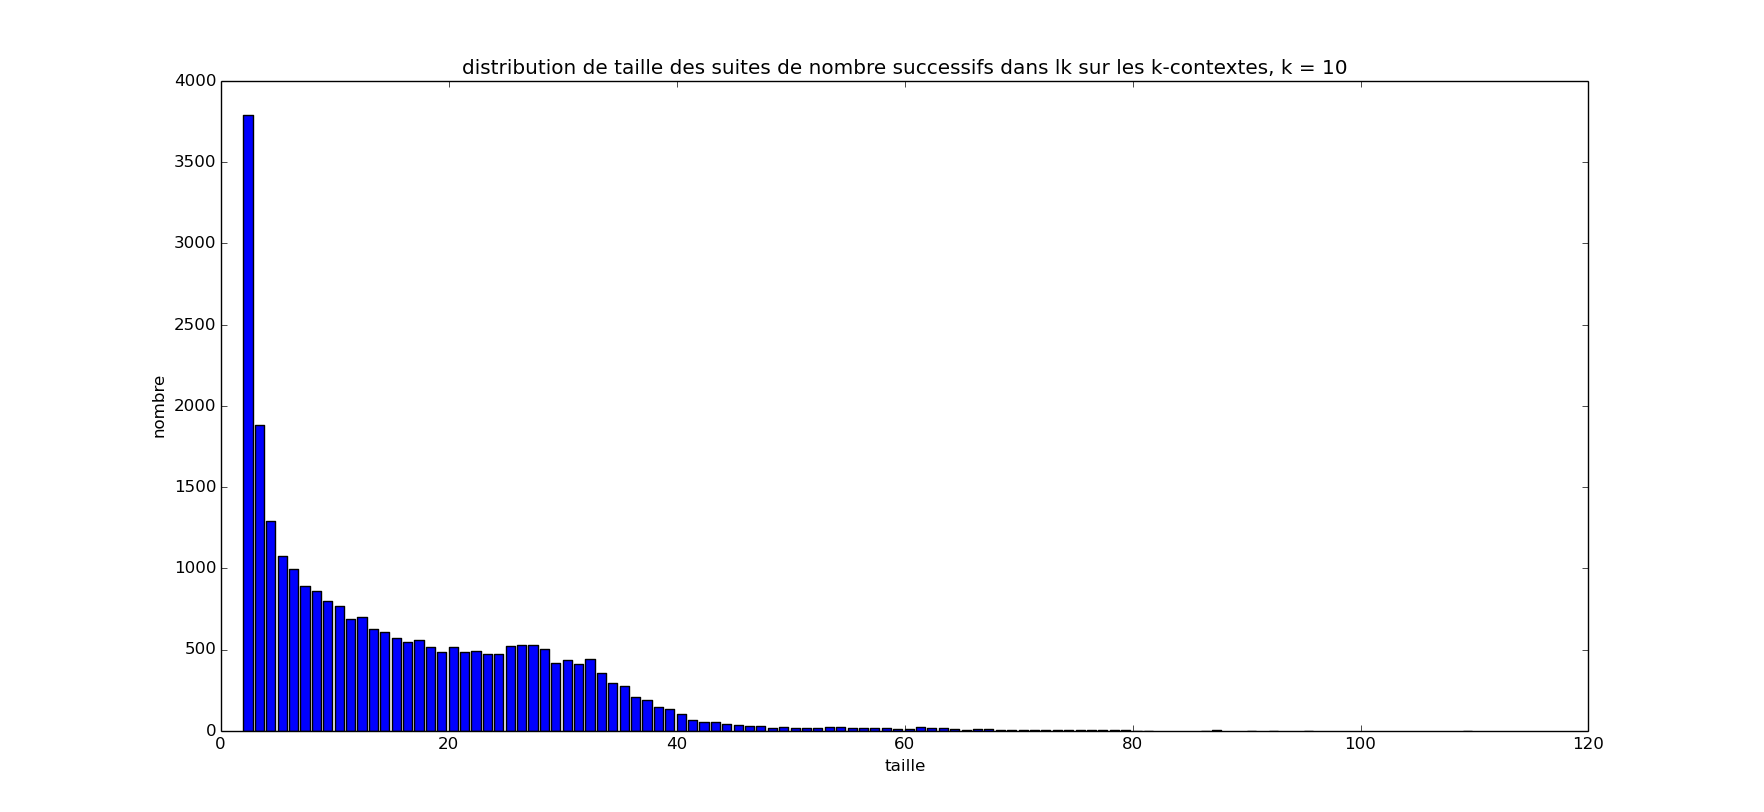
\includegraphics[scale = 0.3]{./images/suitesLFreads10K_k10.png}
    \caption{Distribution de taille des suites de nombres successifs dans LF() sur les k-contextes de la \kbwt\ triée pour $k = 10$ d'un ensemble Reads10K (ensemble de 500 reads de taille 70). On s'aperçoit qu'il y a plus de 7000 suites de nombres successifs supérieures à 20 dans les k-contextes.}
    \label{suitesLF}
\end{figure}

La deuxième approche consiste à regarder la différence entre la fonction LF() et $LF'(i) = C[i] + rank(\bwt[i], i)$, c'est-à-dire la fonction utilisée pour calculer LF() sur la \bwt. Avec cette méthode, il suffit pour retrouver LF() de calculer LF'() et lui ajouter la différence conservée.
%\rmq{S'agit-il de la différence entre LF($i$) et LF'$(i)$ ? Mais dans ce cas, en position i dans la \kbwt{} et dans la BWT nous n'avons pas forcément la même permutation circulaire. Il faut conserver le fait que LF nous amène à la permutation circulaire précédente.}



%
%Premières idées :
%	. chercher par blocs (-> seulement quand bloc assez grand)
%	. stocker permutations (-> infos ne peut pas se contenir elle meme ; décrire différentes idées stockage)

%Implémentation pour tester faisabilité         |  
%étude de la compression                        | -> dans Résultats ?
%calcul de l'entropie pour voir si correspond   | 
%compression avec compresseurs existants        |
%
%pour recherche, besoin de lf. pour lf besoin struc Petri -> lourd
%sur k-contextes, lf croissante -> stocker lf ? mieux
%
%lf lourde
%essais compression
%
%petits k-contextes qd \$ dans contexte -> enlever ces contextes ?
%non

\subsection{Résultats} 

%\textit{Cette section n'est donc pas finie, il manque des résultats dont une partie sur l'entropie, une sur les temps de calcul de recherche des motifs avec le stockage de LF(), et une sur les temps de calcul de la recherche de positions avec l'algorithme 1.}

Pour les résultats de cette section, nous nous sommes appuyés sur un jeu synthétique du génome lambda phage de 500 reads de taille 70, sans erreurs, appelé \textit{reads10K} ; ainsi qu'un jeu plus petit généré artificiellement et toujours sans erreurs, de 400 reads de taille 35, \textit{reads100}.

Nous avons étudié la compression de la \kbwt\ triée par rapport à la \kbwt\ présentée dans la thèse de Petri\up{\cite{petri}}. Comme attendu, on peut voir dans la figure \ref{tailleContextes} que les $k$-contextes de la \kbwt\ pour des reads sont grands et nombreux. La compression est donc meilleure (table \ref{struct}).

\begin{figure}[!ht]
    \center
    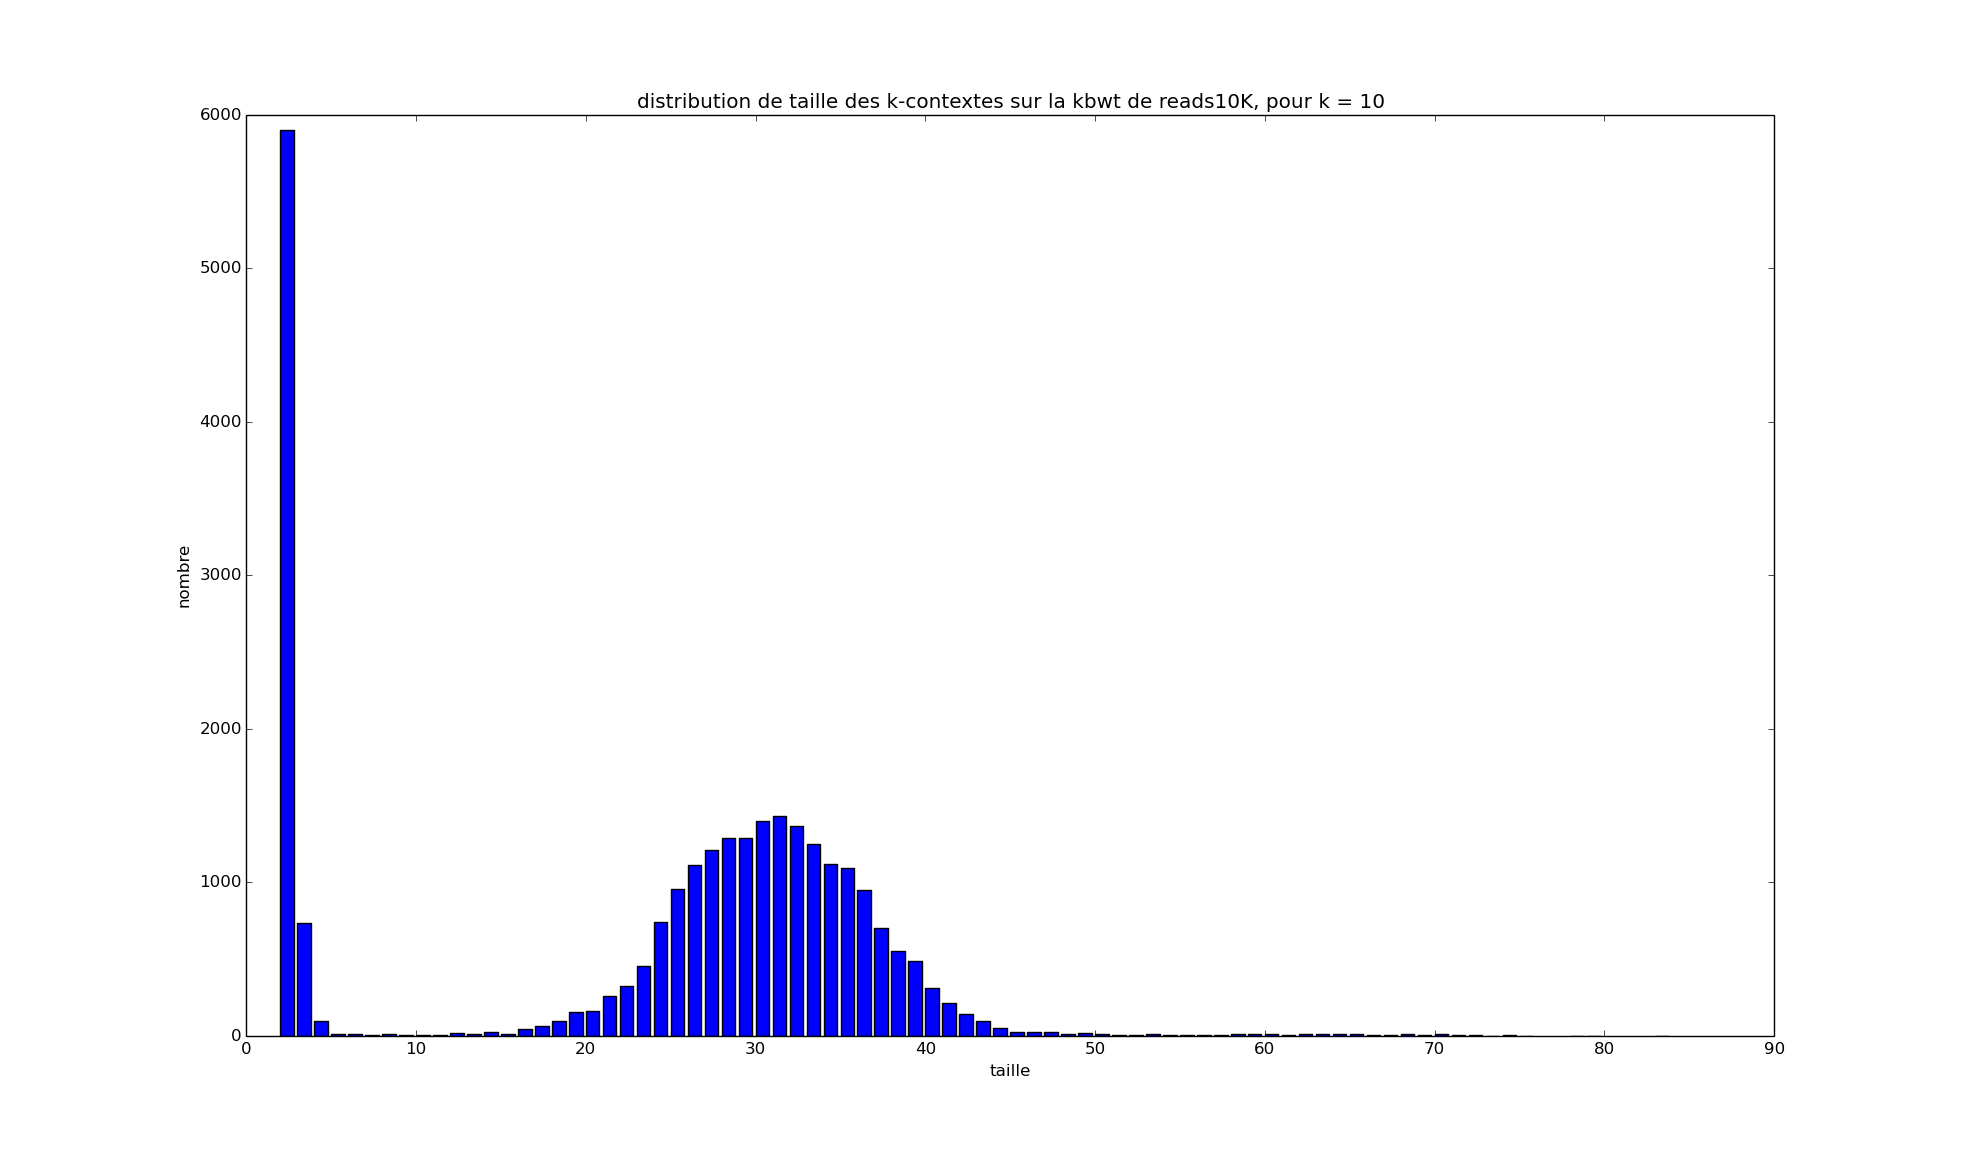
\includegraphics[scale=0.3]{./images/distribReads10K_k10.png}
    \caption{Distribution de taille des $k$-contextes sur la \kbwt\ triée de reads10K, pour $k = 10$. On peut voir que la \kbwt\ triée de cet ensemble comprend environ 15 000 $k$-contextes de taille entre 25 et 40. Les presque 6000 $k$-contextes de taille 2 correspondent aux $k$-contextes chevauchant deux reads.}
    \label{tailleContextes}
\end{figure}

\begin{table}
\centering
\begin{tabular}{|c||c|c|}
	\cline{2-3}
	\multicolumn{1}{c|}{} & reads10K & reads100\\ \cline{2-3} \hline
	fichier original & 51,8~ko & 706~octets\\ \hline
	\bwt & 48,3~ko & 941~octets\\ \hline
	\kbwt & 1,3~ko & 57,3~ko \\ \hline
	\kbwt\ triée & 51,4~ko & 935~octets \\ \hline
	\kbwt\ + $Dk$ & & \\ \hline
	\kbwt\ triée + $Dk$ + $Corr$ & & \\ \hline
\end{tabular}
\caption{Comparaison de la taille des différentes structures étudiées durant ce stage. Les \kbwt\ ont été calculées avec $k=10$. $Dk$ est le vecteur de bits contenant la délimitation des $k$-contextes, $Corr$ est le vecteur de bit introduit dans la section 2.2.1, correspondant au \textit{xor} entre le wavelet tree de la \kbwt\ et celui de la \kbwt\ triée. La compression a été effectuée avec le compresseur \textit{bzip2}.}
\label{struct}
\end{table}

De plus nous avons étudié l'espace pris par la fonction LF() suivant les deux approches décrites dans la section précédente (table \ref{resLF}). On s’aperçoit que la deuxième méthode, la comparaison des deux fonctions LF() et LF'() est légèrement plus compressible. Dans tous les cas, ces méthodes occupent beaucoup moins d'espace que les structures utilisées par Petri.

\begin{table}[h]
\centering
\begin{tabular}{|c|c||c|c|c|c|}
	\cline{3-6}
	\multicolumn{2}{c|}{} & \multicolumn{3}{c|}{reads10K} & reads100\\
	\cline{3-6}
\multicolumn{2}{c|}{}       
& $k=6$  & $k=10$  & $k=20$   & $k=10$ \\ \cline{3-6}\hline
\multicolumn{2}{|c||}{LF()}  
& 1,8~Mo & 1,9~Mo  & 1,2~Mo   & 21,5~ko \\ \hline
\multicolumn{2}{|c||}{LF'()}
& 1,2~Mo & 1,2~Mo  & 1,1~Mo   & 19,9~ko \\ \hline
\multicolumn{2}{|c||}{LF(i+1)-LF(i)} 
\color{red}& 1~Mo   & 1,3~Mo  & 142,2~ko & 5,1~ko  \\ \hline
\multicolumn{2}{|c||}{\color{red}LF()-LF'()}
& \color{red}1,2~Mo & \color{red}84,4~ko & \color{red}101,5~ko & \color{red}4,6~ko  \\ \hline
\multirow{4}{*}{Petri}
& $k-1$-\bwt &   9,5~ko    &   50,5~ko &       52,1~ko &     933~octets \\
& A          &   9,4~ko    &   55,8~ko &       88,9~ko &       1,5~ko \\
& S          &  204,8~ko   &   70,9~ko &       94,2~ko &       1,9~ko \\ \cline{2-6}
& Total &$\geq$~223,7~ko&$\geq$~177,2~ko&$\geq$~235,2~ko&$\geq$~4,3~ko \\ \hline
	
\end{tabular}
\caption{Comparaison de la taille prise par la fonction LF() selon différentes méthodes, pour la \kbwt\ triée de reads10K et reads100. Les dernières lignes du tableau montre l'espace utilisé par l'ensemble des structures utilisées par Petri pour calculer LF() sans la stocker. Seuls les vecteurs de bits ($D_k$ et $D_k-1$) n'ont pas été comptés. La compression a été effectuée avec le compresseur \textit{bzip2}.}
\label{resLF}
\end{table}

